\NEW{
\section{System Overview}
\label{sec:overview}
To optimize inter-DC multicasts on overlay network with dynamical separation with
latency-sensitive traffic, we present {\em \name}, a {\em fully centralized} near-optimal network system with dynamic bandwidth separation for data inter-DC multicast.} Before presenting the details, we first highlight the intuitions behind the design choices, and the challenges behind its realisation.


\mypara{Centralized control}
Conventional wisdom on wide-area overlay networks has relied, to
some extent, on {\em local} adaptation of individual nodes (or
relay servers) to achieve desirable scalability and responsiveness
to network dynamics
(e.g.,~\cite{Andreev2013Designing,Repantis2010Scaling,Huang2014A,mukerjee2014enabling}),
despite the resulting suboptimal performance due to lack of global
view or orchestration.
%Recent work (e.g.,~\cite{mukerjee2014enabling}), however,
%shows the feasibility of combining
%local adaptation with a centralized logic operating
%on coarse timescales.
In contrast, \name takes an explicit stance that it is practical to
fully centralize the control of wide-area overlay networks and
still achieve near-optimal performance in the setting of inter-DC
multicasts. The design of \name coincides with other recent works that centralize the
management of large-scale distributed systems, e.g.,~\cite{gog2016firmament}.
At a high level, \name uses a centralized controller that
periodically pulls information (e.g., data delivery status) from all
servers, updates the decisions regarding overlay routing, and pushes
them to agents running locally on servers
(Figure~\ref{fig:framework}).
Note that when the controller fails or is unreachable, the system will
fall back to a decentralized control scheme to ensure graceful
performance degradation to local adaptation
(\Section\ref{subsec:system:fault}).

\begin{figure}[t]
  \centering
  %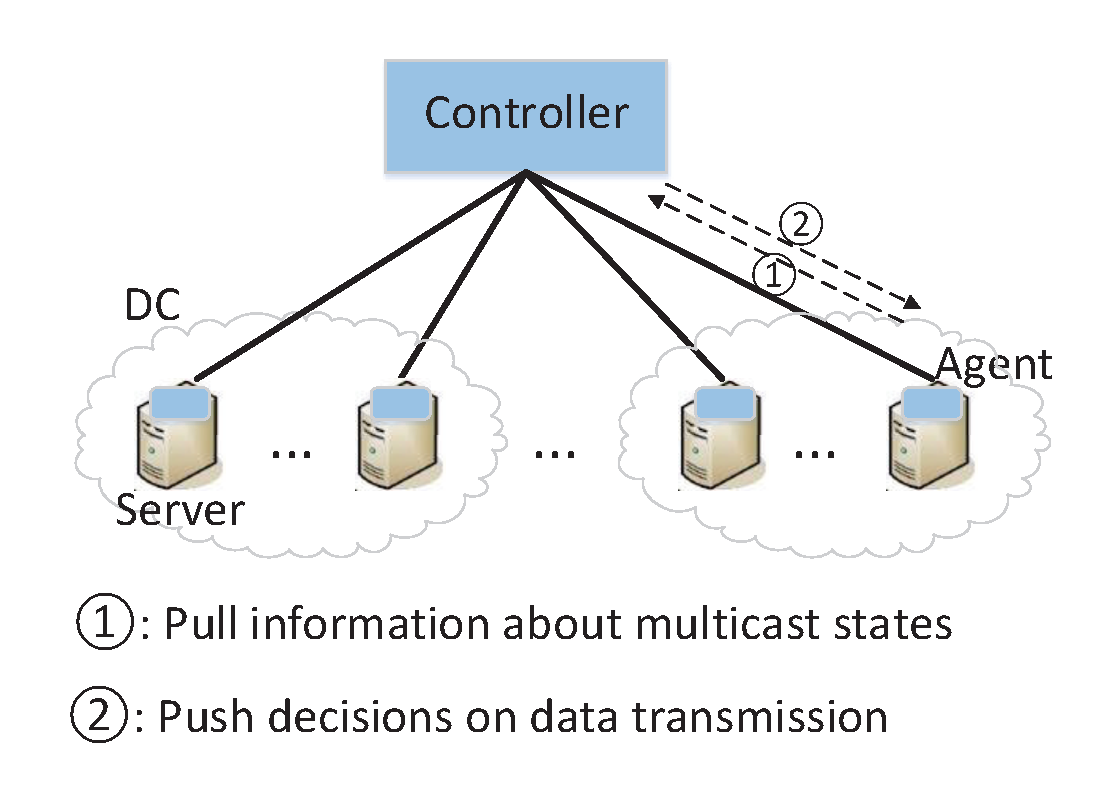
\includegraphics[width=2in]{images/framework.eps}
  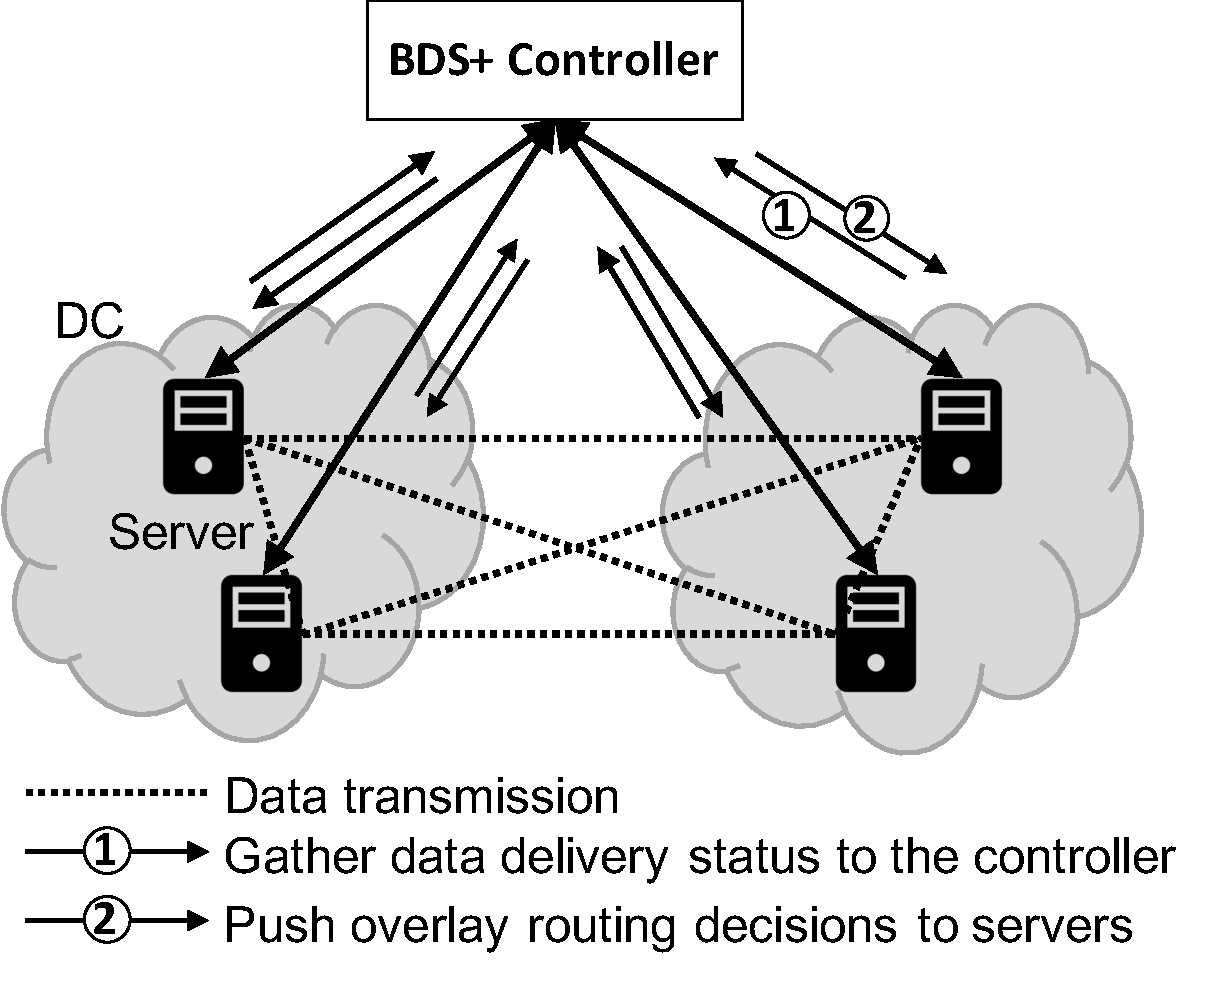
\includegraphics[width=2.3in]{images/framework-journal.pdf}
    \vspace{-0.2cm}
  \tightcaption{The centralized design of \name.}
  \label{fig:framework}
\vspace{-0.4cm}
\end{figure}

Our centralized design is driven by several empirical observations:
\begin{packedenumerate}

\item {\em Large decision space:}
The sheer number of inter-DC overlay paths (which grow exponentially
with the increasing number servers acting as overlay nodes) makes it difficult for
individual servers to explore all available overlay paths based only
on local measurements. In contrast, we could significantly improve
overlay multicast performance by maintaining a global view of data
delivery status of all servers, and dynamically balancing the
availability of various data blocks, which turns out to be critical
to achieving near-optimal performance
(\Section\ref{subsec:logic:scheduling}).

\item {\em Large data size:}
Unlike latency-sensitive traffic which lasts
on timescales of several to 10s of milliseconds, inter-DC multicasts
last on much coarser timescales.
%Thus, it is a necessary requirement to be continously adaptive to
%any transient network dynamics.
%In this context, the tradeoff between a centralized design and a decentralized one is that centralized control essentially trades real-time responsiveness to network dynamics for closer-to-optimal control decisions driven by a global view of data delivery. Here,
Therefore, \name can tolerate a short delay (of a few seconds) in order
to get better routing decisions from a centralized controller which
maintains a global view of data delivery and is capable of orchestrating
all overlay servers.

\NEW{
\item {\em Flexible traffic control:}
\newname can enforce bandwidth allocation by setting limit rates in
each data transfer, while each server can use Linux
Traffic Control (tc) to enforce the limit on the teal bandwidth
usage. This allows \newname to leverage flexible dynamic bandwidth separation. Once any network changes are detected, \name could easily adjust bandwidth for each data transfer by controlling the sending rate at all servers in a centralized fashion (nomatter to reserve more bandwidth when online traffic burst, or to reduce transfer rate when online traffic is in valley). (\Section\ref{sec:deployment}).
%Previous works~\cite{Andreev2013Designing,Repantis2010Scaling,Huang2014A,mukerjee2014enabling} use the static separation scheme where there is a fixed boundary between online and offline traffic, here \name proposes to use dynamic bandwidth separation, so it should know the bandwidth utilization in a global view, in order to dynamically adjust the amount of available bandwidth that can be used for bulk-data transfer.
}

\item {\em Lower engineering complexity:}
Conceptually, the centralized architecture moves the control
complexity to the centralized controller, making \name amenable to a
simpler implementation, in which the control logic running locally in
each server can be stateless and triggered only on arrivals of new
data units or control messages.

\end{packedenumerate}

%\mypara{Fast and near-optimal decision-making}
\mypara{The key to realizing centralized control}
In essence, the design of \name performs a trade-off between incurring
a small update delay in return for the near-optimal
decisions brought by a centralized system. Thus, the key to striking such a
favorable balance is a near-optimal yet efficient overlay routing
algorithm that can update decisions in near realtime. At a first
glance, this is indeed intractable. For the workload at a scale of
\company, the centralized overlay routing algorithm must pick the next
hops for $10^5$ of data blocks from $10^4$ servers. This operates at a scale that
could grow exponentially when we consider the growth in the number of possible
overlay paths that go through these servers and with finer grained
block partitioning. With the standard routing formulation and linear
programming solvers, it could be completely unrealistic to make
near-optimal solutions by exploring such a large decision space
(\Section\ref{subsubsec:evaluation:depth}).

\NEW{
\mypara{The key to realizing dynamic bandwidth separation}
Dynamic bandwidth separation raises two requirements, one is to reserve enough bandwidth for latency-sensitive online traffic so as to avoid negative impacts on these services, and the other is to make full use of the residual bandwidth so as to reduce the completion time of bulk data transfer. With the traditional strict safety threshold and decentralized protocols, it could be impossible to make efficient bandwidth usage in the dynamic and mixed deployed network (\Section\ref{subsec:evaluation:improvements}).
}

The following two sections will present how \name works.

